\documentclass[letterpaper,pdftex]{article}

\setlength{\textwidth}{168mm}
\setlength{\textheight}{210mm}
\setlength{\oddsidemargin}{0cm}
\setlength{\topmargin}{0cm}
\setlength{\headheight}{48pt}
\addtolength{\textheight}{-25pt}
\voffset -0.5in

\usepackage{natbib}
\usepackage[utf8]{inputenc}
\usepackage[spanish]{babel}
\usepackage{xcolor,graphicx}
\usepackage{fancyhdr}
\usepackage{multirow}
\usepackage{hyperref}
\hypersetup{
    colorlinks,
    citecolor=blue,
    filecolor=black,
    linkcolor=blue,
    urlcolor=black
}
\usepackage{epstopdf}
\usepackage[autolinebreaks,useliterate]{mcode}
\pagestyle{fancy}
\renewcommand{\headrule}{\color{gray}
\hrule width\headwidth height\headrulewidth \vskip-\headrulewidth}
\renewcommand{\footrule}{{\color{gray}
\vskip-\footruleskip\vskip-\footrulewidth
\hrule width\headwidth height\footrulewidth\vskip\footruleskip}}
\renewcommand{\headrulewidth}{1.5pt}
\renewcommand{\footrulewidth}{1.5pt}

\usepackage{caption}
\usepackage{subcaption}

\spanishdecimal{.}

\begin{document}
\fancyhead{}
\fancyfoot{}
\fancyhead[L]{
\begin{minipage}{3.5cm}
\begin{center}
	
\includegraphics[width=0.95\textwidth]{logousb.png}
\end{center}
\end{minipage}
\begin{minipage}{12cm}
\begin{flushleft}
\small \textsc{Universidad de San Buenaventura}\\
\small \textsc{Facultad de Ingeniería}\\
\small \textsc{Programa de Ingeniería Mecatrónica\\}
\end{flushleft}
\end{minipage}
}
\fancyhead[R]{
\begin{minipage}{3.0cm}
\begin{flushright}
\small \textsc{Dibujo de \\ Máquinas}\\
\small \textsc{2020-II}
\end{flushright}
\end{minipage}
}
\fancyfoot[R]{\large \textbf{\thepage}}

\begin{minipage}{0.3\textwidth}
\begin{flushleft}
\textbf{Autor:}\\
\textit{Nikolay Prieto Ph.D(c)}\\
\end{flushleft}
\end{minipage}
\begin{minipage}{0.7cm}
\textcolor{gray}{\rule{0.3cm}{2.5cm}}
\end{minipage}
\begin{minipage}{0.64\textwidth}
\Large{\textbf{Laboratorio \\ Dibujo en Ingeniería \\ AutoCAD (Parte I)}}
\end{minipage}\\

\noindent
\textcolor{gray}{\rule{\textwidth}{0.5pt}}\\
\renewcommand{\tablename}{Tabla}
\renewcommand{\arraystretch}{1.2}
\renewcommand\contentsname{Contenido}
\tableofcontents

\noindent
\textcolor{gray}{\rule{\textwidth}{0.5pt}}\\

\section{Introducci\'on}

Diseñar es el proceso de convertir una idea en un objeto, producto o sistema. Este proceso es iterativo. CAD (Computer Aided Design) es una herramienta que se puede utilizar para actividades de diseño y dibujo. Dado que utiliza la potencia informática de un procesador, los dibujos CAD son más rápidos, mejores y más precisos que sus contrapartes redactadas manualmente.

AutoCAD es un software CAD sofisticado que es sinónimo de dibujo de ingeniería. El concepto de AutoCAD evolucionó en la década de 1980, cuando los ingenieros y arquitectos buscaban aprovechar el poder de las computadoras personales recién introducidas para reducir el tiempo de dibujo.

\subsection{Características de AutoCAD}

Cuando decimos ``características'', no nos referimos a los comandos ofrecidos por AutoCAD en el contexto de esta introducción. En su lugar, destacamos las diferencias entre AutoCAD y otro software CAD que hacen de AutoCAD una herramienta de dibujo popular.

\begin{itemize}

\item\textbf{Potente dibujo}: creado principalmente como una herramienta de dibujo, AutoCAD ofrece capacidades de dibujo incomparables.

\item \textbf{Analizar detalles de objetos:} las funciones incluidas en AutoCAD permiten un análisis y visualización en profundidad de modelos 2D y 3D.

\item \textbf{Complementos:} dado que AutoCAD es extremadamente popular, hay una gran cantidad de complementos disponibles que hacen que el software sea más útil y amigable.

\item \textbf{Integración:} AutoCAD permite la integración API con hojas de cálculo, editores de documentos y otras utilidades. Esto es extremadamente útil cuando se comparte la salida del software.

\item \textbf{Opciones de formación}: dado que AutoCAD es muy popular, existen institutos de formación que enseñan el software desde el nivel principiante hasta el nivel avanzado.

\end{itemize}


\section{Ejercicios de Laboratorio}

\subsection{Lineas, círculos y ortogonalidad}

\begin{figure}[h]
     \centering
     \begin{subfigure}[b]{0.45\textwidth}
         \centering
         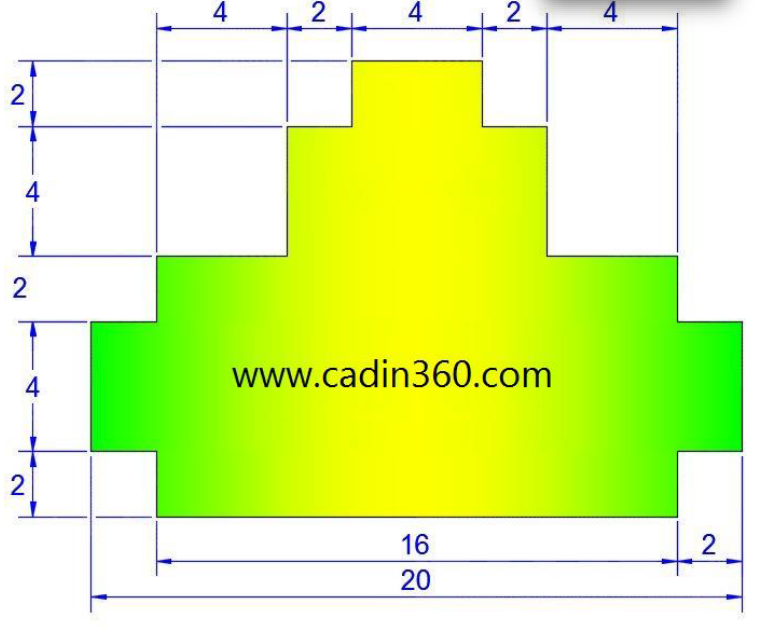
\includegraphics[width=\textwidth]{graph1}
         \caption{Líneas ortogonales}
         \label{fig:simple1}
     \end{subfigure}
     \hfill
     \begin{subfigure}[b]{0.45\textwidth}
         \centering
         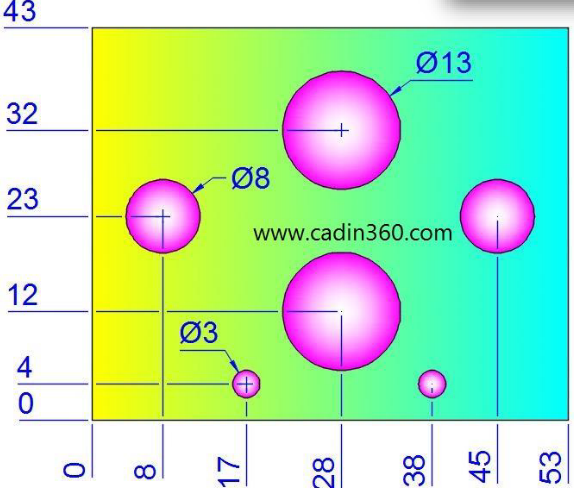
\includegraphics[width=\textwidth]{graph2}
         \caption{Círculos y líneas de centro.}
         \label{fig:simple2}
     \end{subfigure}
\end{figure}

\subsection{semi-círculos, lenguaje de líneas y hatching}

Figuras \ref{fig:simple3} y \ref{fig:simple4}

\begin{figure}[h]
     \centering
     \begin{subfigure}[b]{0.45\textwidth}
         \centering
         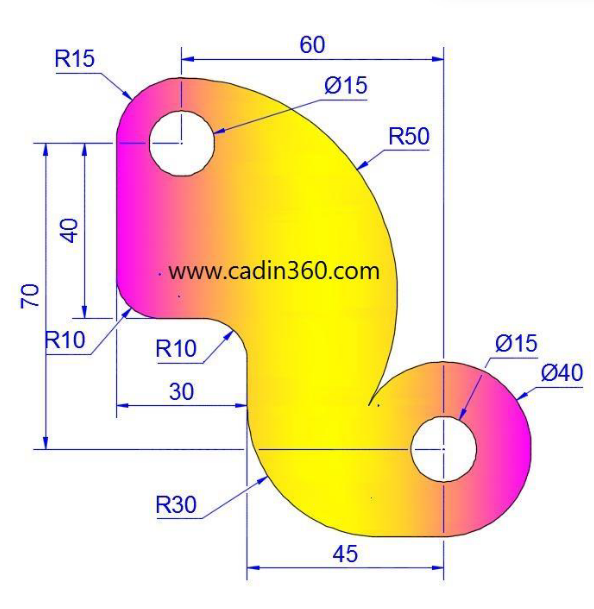
\includegraphics[width=\textwidth]{graph3}
         \caption{semi-círculos tangentes}
         \label{fig:simple3}
     \end{subfigure}
     \hfill
     \begin{subfigure}[b]{0.45\textwidth}
         \centering
         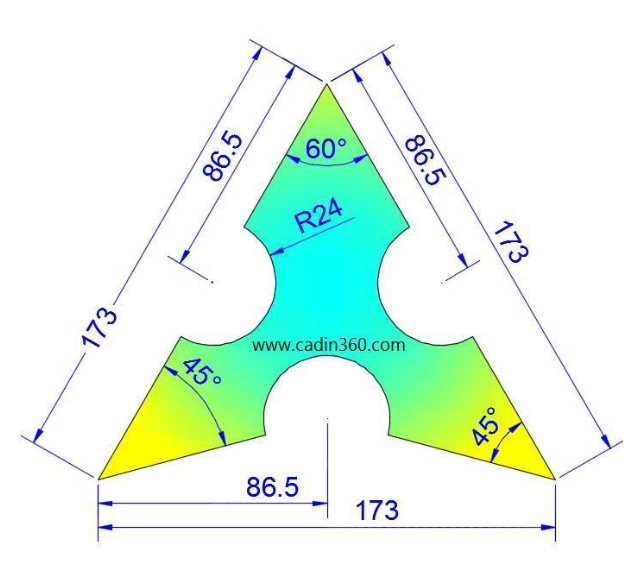
\includegraphics[width=\textwidth]{graph4}
         \caption{Angularidad}
         \label{fig:simple4}
     \end{subfigure}
\end{figure}

\section{Forma de entrega}

Un archivo \textit{.dwg} o \textit{.dxf} usted realizará la entrega del un solo archivo conteniendo los bocetos \ref{fig:der1}, \ref{fig:der2}, \ref{fig:der3}, \ref{fig:der4} y \ref{fig:der5}, 


\begin{figure}[h]
     \centering
     \begin{subfigure}[b]{0.45\textwidth}
         \centering
         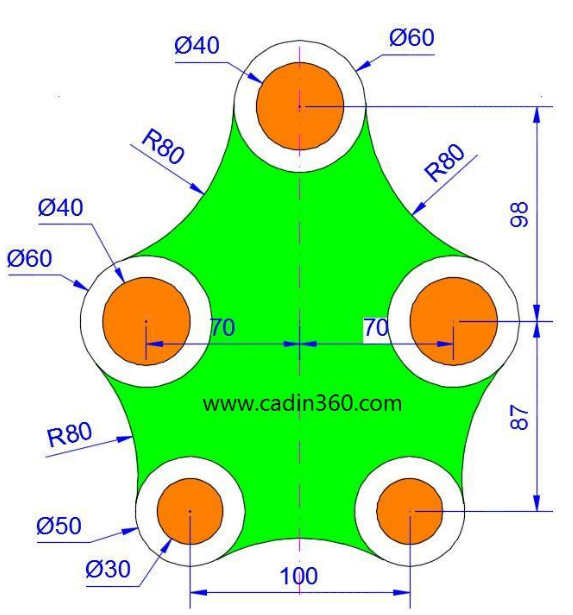
\includegraphics[width=\textwidth]{task1}
         \caption{Entregable 1}
         \label{fig:der1}
     \end{subfigure}
     \hfill
     \begin{subfigure}[b]{0.45\textwidth}
         \centering
         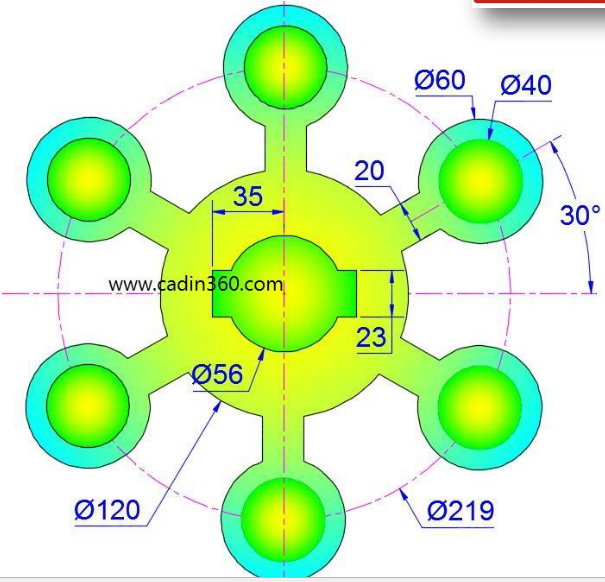
\includegraphics[width=\textwidth]{task2}
         \caption{Entregable 2}
         \label{fig:der2}
     \end{subfigure}
\end{figure}
%
\begin{figure}[h]
     \centering
     \begin{subfigure}[b]{0.45\textwidth}
         \centering
         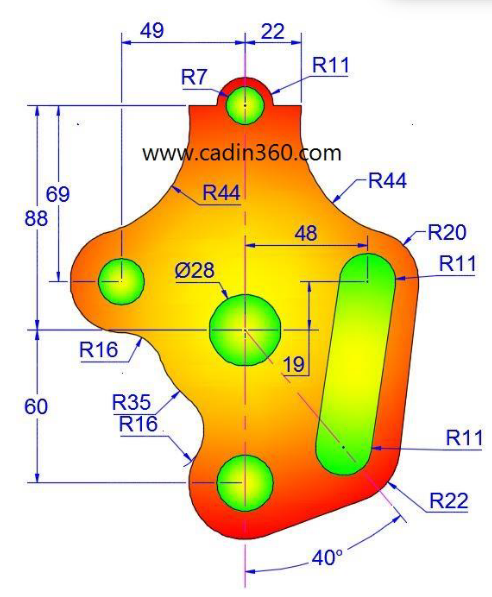
\includegraphics[width=\textwidth]{task3}
         \caption{Entregable 3}
         \label{fig:der3}
     \end{subfigure}
     \hfill
     \begin{subfigure}[b]{0.45\textwidth}
         \centering
         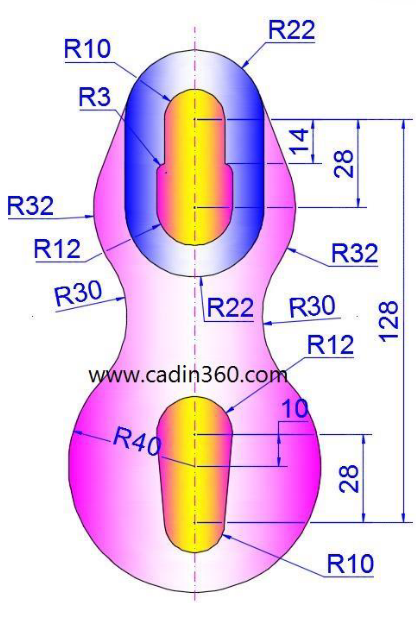
\includegraphics[width=\textwidth]{task4}
         \caption{Entregable 4}
         \label{fig:der4}
     \end{subfigure}
\end{figure}
%
\begin{figure}[h]
   \centering
   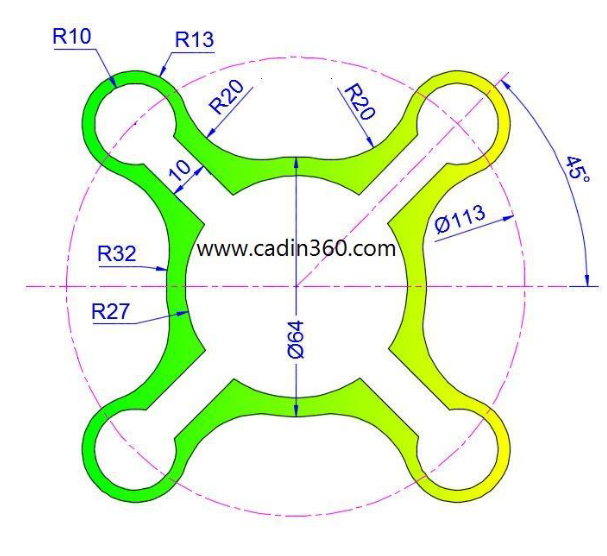
\includegraphics[width=0.6\textwidth]{task5}
   \caption{Entregable 5}
   \label{fig:der5}
\end{figure}

\end{document}
